\documentclass[a4paper,12pt,floatssmall]{scrartcl}

% Page geometry's formatting
\usepackage[left=2.5cm,right=2.5cm,top=2.5cm,bottom=2.5cm]{geometry}
\usepackage{indentfirst}
\usepackage{placeins}
\usepackage{float}
% Language-specific settings
\usepackage[T1]{fontenc}
\usepackage[utf8]{inputenc}
\usepackage[polish]{babel}
\usepackage{polski}
% Elements' embedding
\usepackage{listings}
\usepackage{graphicx}
\usepackage[bf]{caption}
\usepackage{subcaption}
\usepackage{hyperref}
% Text-formatting
\usepackage[autostyle]{csquotes}
\usepackage{caption}
\usepackage{moresize}
\usepackage{amsmath}
% Miscellaneous
\usepackage[backend=biber,style=ieee]{biblatex}
\usepackage[enable]{easy-todo}
\usepackage{lipsum}
\usepackage{setspace}


% ============================================================================================================== %
% ----------------------------------------------- Configuration ------------------------------------------------ %
% ============================================================================================================== %

% Unordered list
\renewcommand{\labelitemi}{\textbullet}

% Bibliography file
\addbibresource{bibliography.bib}

% ============================================================================================================== %
% --------------------------------------------- Macrodefinitions ----------------------------------------------- %
% ============================================================================================================== %

% Redefininiton of the title page
\renewcommand{\maketitle}{
\begin{titlepage}
    \vfill
    \begin{center}
        \begin{figure}
            \centering
            
\includegraphics[scale=0.9]{img/header.png}
            \vspace{0.5cm}
        \end{figure}
    \end{center}
    \vspace{2cm}
    \begin{center}
        {\HUGE {\textbf{Programowanie kładów FPGA}}}\\
        \vspace {0.4cm}
        {\Large {(projekt)}}
    \end{center}
    \vspace{4cm}
    \begin{center}
        {\setstretch{1.5}\textbf{\LARGE Implementacja algorytmów cyfrowego przetwarzania sygnałów audio na bazie układu FPGA z interfejsem UART}}
        \vspace{3cm}
    \end{center}
    \vfill
    \begin{center}
        {\textbf{\normalsize Pierczyk Krzysztof}}
    \end{center}
    \vfill
    \begin{center}
        \large{Warszawa, \today \par}
    \end{center}
\end{titlepage}
}


% ============================================================================================================== %
% --------------------------------------------------- Text ----------------------------------------------------- %
% ============================================================================================================== %

\begin{document}
    
% Title
\maketitle

% Table of content
\tableofcontents
\clearpage

% Content
\section{Wstęp}

Celem projektu jest opracowanie i~zaimplementowanie zestawu wybranych metod przetwarzania sygnałów audio znanych z~popularnych multiefektów gitarowych. Zadaniem tego typu rozwiązań jest modyfikowanie próbkowanego dźwięku w~czasie rzeczywistym w taki sposób, aby urozmaicić jego brzmienie np. poprzez modulację, przesunięcie fazowe lub wprowadzenie dodatkowych składowych. Przykładami takich efektów są m.in.

\begin{itemize}
    \item \textbf{echo} (opóźnienie, ang. \textit{delay}) - do sygnału dodawana jest jedna lub kilka jego kopii opóźnionych o~określoną liczbę próbek; efekt ma symulować warunki panujące w~halach widowiskowych
    \item \textbf{overdrive} - nazwa ogółu metod prowadzących do znacznego zniekształcenia sygnału bazowego; jednym z~popularnych sposobów jego implementacji jest nałożenie obustronnych ograniczeń na wyjściowe wartości przepuszczanego sygnału
    \item \textbf{flanger} - kolejny efekt wykorzystujący opóźnione próbki sygnału; w~tym przypadku wielkość opóźnienia podlega cyklicznym zmianom, co przekłada się na pulsacyjny charakter wyjściowego dźwięku
    \item \textbf{tremolo} - efekt modulujący amplitudę sygnału zgodnie z~przebiegiem pewnej funkcji okresowej (np. sinus lub fala trójkątna); jego celem jest symulowanie rodzaju artykulacji polegającego na szybkim wydobywaniu dźwięków o~tej samej częstotliwości (np. poprzez szybkie szarpanie pojedynczej struny gitarowej) 
\end{itemize}

Powyższe efekty stanowią jedynie niewielki wycinek stosowanych rozwiązań, wśród których wymienić można także szeroko pojęte metody equalizacji, czy modyfikowania częstotliwości sygnału. Minimalna wersja projektu zakłada implementację scharakteryzowanych metod przetwarzania wraz z~prostymi mechanizmami wprowadzania i~wyprowadzania danych z~urządzenia a~także dostosowywania parametrów filtrów. Jako metodę komunikacji wybrano popularny (choć może w~niec innych zastosowaniach) interfejs UART (ang. \textit{universal asynchronous receiver-transmitter}). Jego prostota umożliwi przyspieszenie procesu implementacji, a~co za tym idzie szybsze przejście do zasadniczej części projektu. Cyfrowy charakter UARTa pozwoli w~przyszłości przejść na popularny interfejs $I^{2}S$, dzięki któremu możliwe będzie proste dołączenie do urządzenia układów przetwornikowych. Testowanie urządzenia obywać się będzie z~pomocą prostej aplikacji w~języku Python, która za pośrednictwem wirtualnego portu szeregowego wysyłać będzie do urządzenia próbki dźwięku. Sygnał wychodzący z~układu FPGA będzie następnie odtwarzany za~pomocą jednej z~wielu dostepnych w~Pythonie bibliotek audio jak np. \verb|pyaudio|.

\section{Analiza interfejsu komunikacyjnego}

Interfejs UART jest dzisiaj dostępny w~niemal wszystkich obecnych na mikrokontrolowerowych oraz w~wielu układach typu SoC. Jego popularność wynika zarówno z~(jak sama nazwa wskazuje) uniwersalnego charakteru jak i~prostoty implementacji. UART to cyfrowe urządzenie peryferyjne umożliwiające szeregową komunikację asynchroniczną. W~większości implementacji parametry komunikacji takie jak szybkość, czy format danych mogą być konfigurowane poprzez zmianę wartości odpowiednich rejestrów sterujących. Nierzadko możliwe jest też ustawienie trybu komunikacji spośród \textit{simplex}, \textit{duples} lub ~\textit{half-duples}. Interfejsy tego typu, szczególnie w~zastosowaniach przemysłowych, są często sprzęgane z~konwerterami poziomów logicznych odpowiednich dla standardów RS-232 lub RS-485.

\begin{figure}
    \centering
    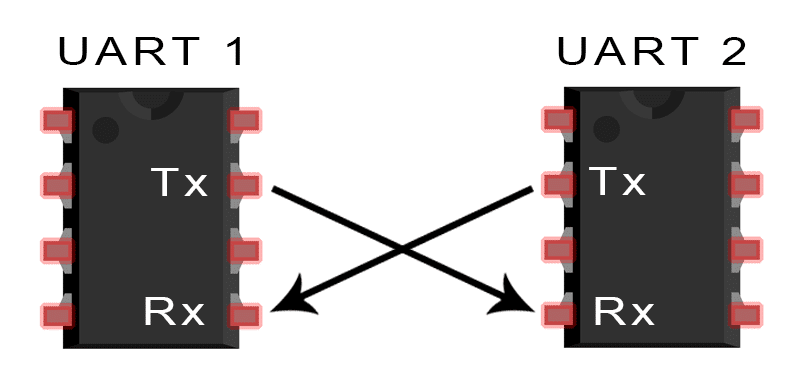
\includegraphics[scale=0.5]{img/uart.png}
    \captionsetup{format=plain,justification=centering}
    \caption{Typowa struktura komunikacji dwóch węzłów z~wykorzystaniem układu UART, źródło: \cite{uart}}
    \label{UART}
\end{figure}

Komunikacja asynchroniczna wymaga aby wszystkie węzły nadawały i~odbierały dane o~z~góry ustalonym formacie i~długości znaku (wynikającym z~szybkości transmisji). Ponadto należy wziąć pod uwagę, że zegary obecne w~poszczególnych urządzeniach mogą się z~czasem rozsynchronizowywać, a~co za tym idzie konieczny jest mechanizm ponownej synchronizacji. W~przypadku komunikacji z~wykorzystaniem modułu UART mechanizm ten wynika z~formatu przesyłanych danych. Typowa ramka składa się z~trzech elementów: \textbf{bitu startu}, \textbf{bitów danyc} oraz \textbf{bitów stopu}. Bit startu oznacza początek nowej ramki i~jest sygnalizowany stanem niskim na linii. Po nim następować może pewna liczba bitów danych - zazwyczaj $7$ lub $8$  - a~na końcu jeden lub dwa bity stopu (sygnalizowane stanem wysokim). Bit startu odpowiada za synchronizację zegarów wykorzystywanych do próbkowania stanu linii, natomiast bity stopu definiują minimalną przerwę między kolejnymi ramkami. Fakt że każdy bit startu to ponowna okazja do zsynchronizowania zegarów sprawia, że nie muszą one pracować z~dokładnie tymi samymi szybkościami. Niewielkie różnice nie powodują błędów w~odbiorze danych.

\begin{figure}
    \centering
    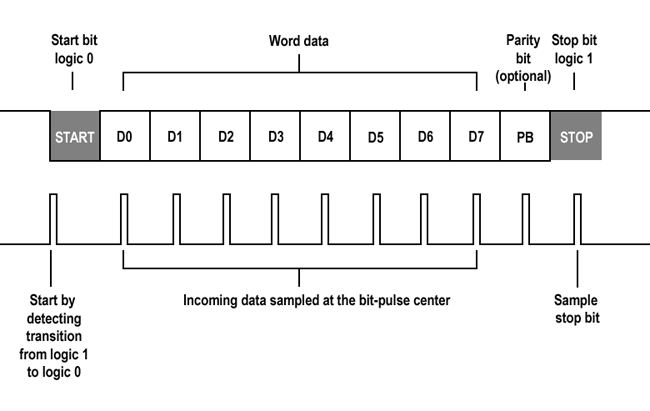
\includegraphics[scale=0.5]{img/uart_frame.png}
    \captionsetup{format=plain,justification=centering}
    \caption{Struktura ramki UART, źródło: \cite{uart_frame}}
    \label{UART}
\end{figure}

Format ramki może zostać rozszerzony o~element kontrolny w~postaci \textbf{bitu parzystości}. Jeśli występuje, przyjmuje on wartość zależną od ilości bitów w~stanie wysokim w~przesyłanych danych i~znajduje się przed bitami stopu. Możliwy jest bit parzystości (ang. \textit{even}) - ustawiony, gdy suma jest parzysta - lub nieparzystości (ang. \textit{odd}) - ustawiany, gdy suma jest nieparzysta. Dodatkowy element pozwala wykrywać ewentualne błędy transmisji. Format ramki często oznacza się w~postaci trzyznakowego identyfikatora postaci $DPS$, gdzie $D$ oznacza ilość bitów danych, $P$ - typ bitu kontrolnego ($E$ - bit parzystości, $O$ - bit nieparzystości, $N$ - brak bitu kontrolnego) a~$S$ ilość bitów stopu. Typowowymi prędkościami transmisji przez UART są:

\begin{itemize}
    \item 9600 bit/s
    \item 19200 bit/s
    \item 38400 bit/s
    \item ...
\end{itemize}

Jest to pewna zaszłość historyczna wynikająca z~częstotliwości standardowych oscylatorów dostępnych na rynku. Moduły współcześnie implementowane w~układach scalonych wzbogacone są często o~dodatkowe wyprowadzenia zegarowe umożliwiające komunikację synchroniczną. Tego typu urządzenia określane są zazwyczaj mianem USART (ang. \textit{universal synchronous asynchronous receiver-transmitter}).


\end{document}


